



\documentclass{article}

\usepackage{fancyhdr}
\usepackage{extramarks}
\usepackage{amsmath}
\usepackage{amsthm}
\usepackage{amsfonts}
\usepackage{tikz}
\usepackage{enumerate}
\usepackage{graphicx}
\graphicspath{ {images/} }
\usepackage[plain]{algorithm}
\usepackage{algpseudocode}
\usepackage[document]{ragged2e}
\usepackage{textcomp}
\usepackage{color}   %May be necessary if you want to color links
\usepackage{import}
\usepackage{natbib}
\usepackage{hyperref}
\hypersetup{
    colorlinks=true, %set true if you want colored links
    linktoc=all,     %set to all if you want both sections and subsections linked
    linkcolor=black,  %choose some color if you want links to stand out
}

\usetikzlibrary{automata,positioning}


% Basic Document Settings


\topmargin=-0.45in
\evensidemargin=0in
\oddsidemargin=0in
\textwidth=6.5in
\textheight=9.0in
\headsep=0.25in
\setlength{\parskip}{1em}

\linespread{1.1}

\pagestyle{fancy}
\lhead{\hmwkAuthorName}
\lfoot{\lastxmark}
\cfoot{\thepage}

\renewcommand\headrulewidth{0.4pt}
\renewcommand\footrulewidth{0.4pt}

\setlength\parindent{0pt}


\newcommand{\hmwkTitle}{Math 425B Midterm 1 Cheat Sheet}
\newcommand{\hmwkAuthorName}{\textbf{G. Faletto} }


%%%%% Title Page


\title{
    \vspace{2in}
    \textmd{\textbf{ \hmwkTitle}}\\
}

\author{Gregory Faletto}
\date{}

\renewcommand{\part}[1]{\textbf{\large Part \Alph{partCounter}}\stepcounter{partCounter}\\}


%%%%% Various Helper Commands


%%%%% Useful for algorithms
\newcommand{\alg}[1]{\textsc{\bfseries \footnotesize #1}}

%%%%% For derivatives
\newcommand{\deriv}[2]{\frac{\mathrm{d} #1}{\mathrm{d} #2}}

%%%%% For partial derivatives
\newcommand{\pderiv}[2]{\frac{\partial #1}{\partial #2}}

%%%%% Integral dx
\newcommand{\dx}{\mathrm{d}x}

%%%%% Alias for the Solution section header
\newcommand{\solution}{\textbf{\large Solution}}

%%%%% Probability commands: Expectation, Variance, Covariance, Bias
\newcommand{\E}{\mathbb{E}}
\newcommand{\Var}{\mathrm{Var}}
\newcommand{\Cov}{\mathrm{Cov}}
\newcommand{\Bias}{\mathrm{Bias}}
\newcommand\indep{\protect\mathpalette{\protect\independenT}{\perp}}
\def\independenT#1#2{\mathrel{\rlap{$#1#2$}\mkern2mu{#1#2}}}
\DeclareMathOperator{\Tr}{Tr}

\theoremstyle{definition}
\newtheorem{theorem}{Theorem}
\theoremstyle{definition}
\newtheorem{proposition}[theorem]{Proposition}
\theoremstyle{definition}
\newtheorem{lemma}[theorem]{Lemma}
\theoremstyle{definition}
\newtheorem{corollary}{Corollary}[theorem]
\theoremstyle{definition}
\newtheorem{definition}{Definition}[section]
\newtheorem*{remark}{Remark}
\theoremstyle{definition}
\newtheorem{exercise}{Exercise}
\theoremstyle{definition}
\newtheorem{example}{Example}[section]

%%%%% Tilde
\newcommand{\textapprox}{\raisebox{0.5ex}{\texttildelow}}

\begin{document}

\maketitle

\pagebreak

%\tableofcontents

%\
%
%\
%
%\begin{center}
%Last updated \today
%\end{center}



\newpage


\section{Function Spaces: Uniform Convergence and \(C^0\) (Chapter 4 of \citet{pugh2015real}, Section 4.1)}

\begin{definition}[\textbf{Pointwise convergence; from Section 4.1 of \citet{pugh2015real}}]

Let \(\mathcal{X}\) be a set, let \((\mathcal{Y}, d)\) be a metric space. Let \(f_n : \mathcal{X} \to \mathcal{Y}\) be functions for \(n \geq 1\). Let \(f: \mathcal{X} \to \mathcal{Y}\) be another function. We say \textbf{\(f_n\) converges to \(f\) pointwise} if for all \(x \in \mathcal{X}\), the sequence \(\{ f_n(x)\}_{n=1}^\infty\) converges to \(f(x)\) as a sequence of points in \(\mathcal{Y}\). I.e., if for all \(\epsilon > 0\) and for all \(x \in \mathcal{X}\), there exists \(N\) (maybe depending on \(\epsilon\) and \(x\)) such that for \( n \geq N\), we have \(d(f_n(x), f(x)) < \epsilon\). 

\end{definition}

\begin{definition}[\textbf{Uniform convergence; from Section 4.1 of \citet{pugh2015real}}]

Let \(\mathcal{X}\) be a set, let \((\mathcal{Y}, d)\) be a metric space. Let \(f_n : \mathcal{X} \to \mathcal{Y}\) be functions for \(n \geq 1\). Let \(f: \mathcal{X} \to \mathcal{Y}\) be another function. We say \textbf{\(f_n\) converges uniformly to \(f\)} if for all \(\epsilon > 0\), there exists \(N\) (maybe depending on \(\epsilon\) bit not \(x\)) such that for \( n \geq N\) and for all \(x \in \mathcal{X}\), we have \(d(f_n(x), f(x)) < \epsilon\). 

\end{definition}

\begin{remark}

Note that uniform convergence implies pointwise convergence. This fact implies that uniform limits are unique, since limits in metric space \((\mathcal{Y}, d)\) are unique, so the pointwise limits of sequences of functions are unique. 

\end{remark}


\begin{example}[\textbf{Example from 4.1 of pointwise convergence but not uniform convergence.}]\label{ex.pugh.4.1.pt.convg}

\begin{proposition} In Example \ref{ex.pugh.4.1.pt.convg}, \(f_n\) does not converge uniformly to \(f\).

\end{proposition}

\begin{proof}

Suppose \(f_n\) converges uniformly to 0 (the pointwise limit). Take \(\epsilon = 1/2\). Can choose \(N \geq 1\) such that  \(|x^n - 0 | < 1/2\) for all \(n \geq N\), and for all \(x \in (0,1)\). Let \(x = (3/4)^{1/N}\). (\(N\)th roots exist by IVT.) Then \(|x^N - 0| = 3/4 \) which is not less than 1/2. 

\end{proof}

\end{example}


\begin{theorem}[\textbf{Cauchy 1821; Theorem 4.1 from \citet{pugh2015real}}]\label{ra.thm.41.pugh}

Let \((X,d)\) and \((Y, d')\) be metric spaces. Let \(f_n: X \to Y\) be continuous at \(x_0 \in X\) for all \(n \geq 1\). Suppose \(f_n\) converges uniformly to \(f\) for some \(f:X \to Y\). Then \(f\) is continuous at \(x_0\). (This implies that if all \(f_n\) are continuous everywhere and \(f_n\) converges uniformly to \(f\) then \(f\) is continuous everywhere.)

\end{theorem}


What about if you only have pointwise convergence? Then this theorem won't work. Consider the sawtooth wave example: the limit is not continuous. There exist easier counterexamples as well.

\begin{example}[From Section 4.1, p. 212 of \citet{pugh2015real}]

Let \(X = [0,1]\), \(Y = \mathbb{R}\), \(f_n(x) = x^n\). Let \(f:[0,1] \to \mathbb{R}\) be defined by 

\[
f(x) = \begin{cases}
0, & 0 \leq x < 1, \\
1, & x=1
\end{cases}
\]

As before, \(f_n\) converges to \(f\) pointwise but not uniformly. \(f_n\) is continuous on \([0,1]\) for all \(n\) but \(f\) is not. See Figure \ref{ra.fig.88}.

\begin{figure}[htbp]
\begin{center}
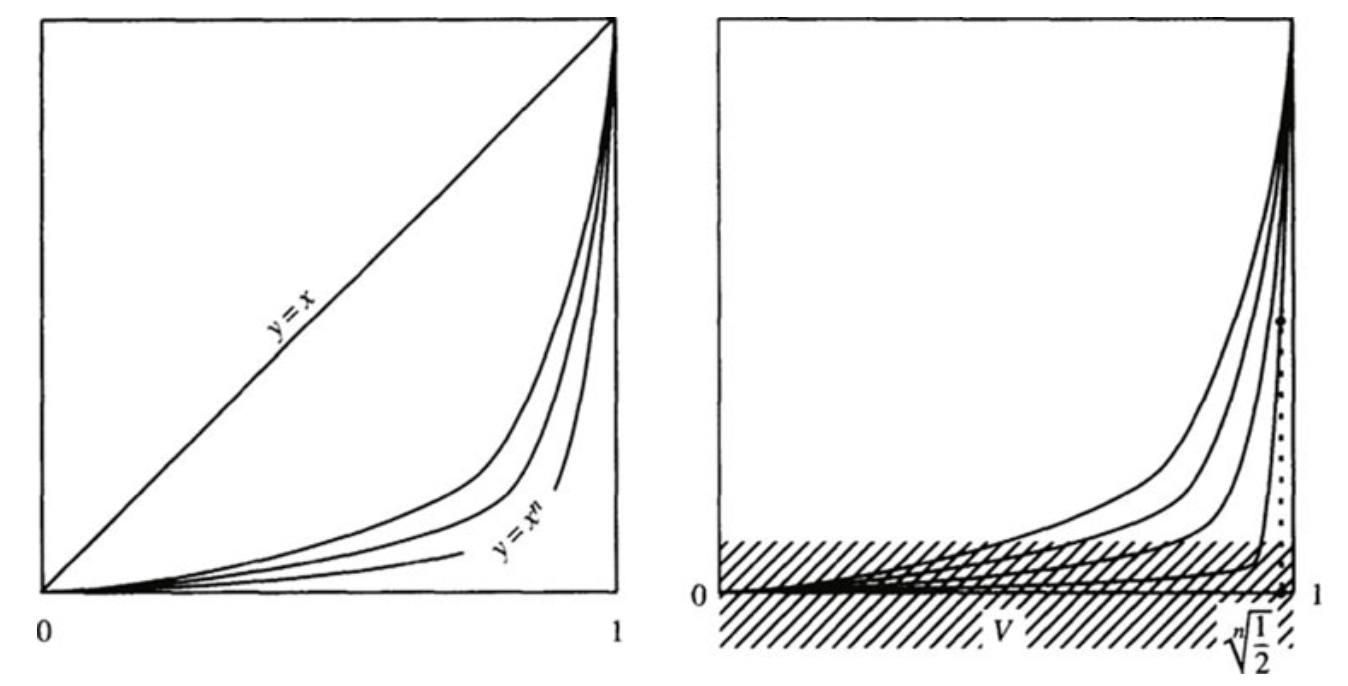
\includegraphics[scale=0.5]{ra_fig88}
\caption{Figure 88 from Section 4.1, p. 213 of \citet{pugh2015real}}
\label{ra.fig.88}
\end{center}
\end{figure}


\end{example}

\begin{exercise}\label{ra.425b.bounded}

Let \(X\) be a set, \((Y, d)\) be a metric space. Let \(x_0 \in X\) be fixed. Let \(f: X \to Y\) be a function. Then the following are equivalent:

\begin{enumerate}

\item There exists \(m \in \mathbb{R}\) such that \(d(f(x_0), f(x)) \leq m\) for all \(x \in X\). 

\item There exists \(x_1 \in X\) and \(m \in \mathbb{R}\) such that \(d(f(x_1), f(x_2)) \leq m\) for all \(x_2 \in X\).

\item There exists \(m \in \mathbb{R}\) such that \(d(f(x_1), f(x_2)) \leq m\) for all \(x_1, x_2 \in  X\). 

\end{enumerate}

\end{exercise}

\begin{definition}

If \(f:X \to (Y, d)\) satisfies the statements in Exercise \ref{ra.425b.bounded}, then \(f\) is called \textbf{bounded.}

\end{definition}

\begin{definition}

Let \(X\) be a set and \((Y,d)\) be a metric space. Define \(C_b(X,Y)\) as the set of bounded functions from \(X\) to \(Y\). 



\end{definition}


\begin{definition}

For \(f, g \in C_b(X, Y)\), let \(d_\infty(f, g) := \sup_{x \in X} d(f(x), g(x))\). 

\end{definition}



\begin{theorem}[\textbf{Theorem 4.2 in \citet{pugh2015real}}]

\(X\) set, \((Y,d)\) metric space. If \(f_n \in C_b(X, Y)\) for \(n \geq 1\) and \(f \in C_b(X, Y)\), then \(f_n\) converges uniformly to \(f\) if and only if \(f_n \xrightarrow{d_\infty} f)\). 

\end{theorem}

\begin{proposition}[Uniform convergence preserves boundedness]

If \(f_n: X \to Y\) is bounded for all \(n\) and \(f_n\) converges uniformly to \(f\), then \(f\) is bounded.

\end{proposition}

\begin{corollary}[\textbf{similar to Theorem 4.2 in \citet{pugh2015real}}]

If \(f_n \in C_b(X, Y)\) for \(n \geq 1\), then \((f_n)\) converges uniformly if and only if \((f_n)\) converges in \(C_b(X, Y)\). (functional analysis perspective of uniform convergence.)

\end{corollary}

\begin{definition}

\(X\) set, \((Y,d)\) metric space. A sequence of functions \(f_n: X \to Y\) is \textbf{uniformly Cauchy} if for every \(\epsilon >0\) there exists \(N \geq 1\) such that for \(n, m \geq N\) we have \(d(f_n(x), f_m(x)) < \epsilon\) for all \(x \in X\).

\end{definition}


\begin{theorem}\label{ra.thm.tricky}

\(X\) set, \((Y,d)\) metric space. If \((Y, d)\) is complete, then any uniformly Cauchy sequence of functions \(f_n: X \to Y\) is uniformly convergent.

\end{theorem}


\begin{definition}

Assume both \((X, d)\) and \((Y, d')\) are metric spaces. \((C^0(X,Y) \subset C_b(X,Y)\) is the set of bounded continuous functions \(X \to Y\). We can restrict \(d_\infty\) to \(C_0(X,Y)\) and get a metric subspace.

\end{definition}


\begin{corollary}[\textbf{Corollary to Theorem \ref{ra.thm.41.pugh}}]\label{ra.thm.41.pugh.cor2}

\(C^0(X,Y)\) is a closed subset of \(C_b(X,Y)\).

\end{corollary}


\bibliographystyle{abbrvnat}
\bibliography{mybib2fin}


\end{document}